\RequirePackage[l2tabu, orthodox]{nag}

\documentclass[border=10pt]{standalone} 
\usepackage[latin1]{inputenc}
\usepackage[english]{babel}
\usepackage{mathptmx}

\usepackage[doublespacing]{setspace}
\usepackage[left=2.5cm,right=2.5cm,top=2.5cm,bottom=2.5cm]{geometry}

\usepackage{natbib}
\usepackage{amsmath}
\numberwithin{equation}{section}

\usepackage{array}
\usepackage{booktabs} 
\usepackage{tabularx}
\newcolumntype{L}[1]{>{\raggedright\arraybackslash}p{#1}} % linksbündig mit Breitenangabe
\usepackage[pdftex]{hyperref}  
%\usepackage{todonotes}

\usepackage{tikz}
\usetikzlibrary{arrows,calc}
\usetikzlibrary{arrows,automata,shapes.geometric}
\usetikzlibrary{positioning}
\tikzset{
>=stealth',
help lines/.style={dashed, thick},
axis/.style={<->},
important line/.style={thick},
connection/.style={thick, dotted},
}
\tikzset{
    state/.style={
           rectangle,
           rounded corners,
           draw=black, very thick,
           minimum height=2em,
           inner sep=2pt,
           text centered,
           },
}
\newenvironment{keywords}%
   {\begin{trivlist}\item[]{\bfseries\sffamily Keywords:}\ }
   {\end{trivlist}}
   
\usepackage{microtype}

\begin{document}


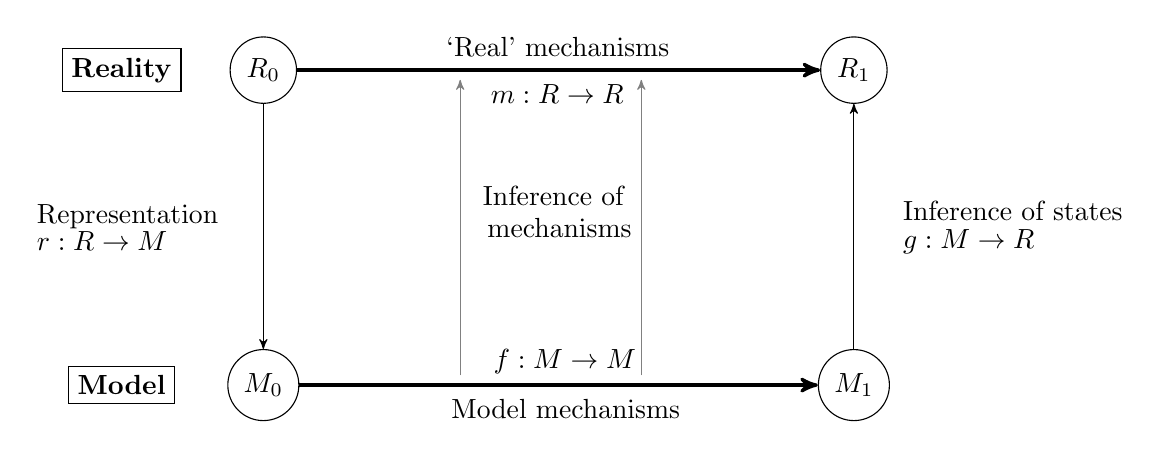
\begin{tikzpicture}[->,>=stealth', scale=0.5]
\node[draw,circle, xshift=-1cm, yshift=3cm] (r) {$R_0$};
\node[draw,circle, xshift=-1cm, yshift=-1cm] (m) {$M_0$};
\node[draw,circle, xshift=6.5cm, yshift=3cm] (r1) {$R_1$};
\node[draw,circle, xshift=6.5cm, yshift=-1cm] (m1) {$M_1$};
\node[xshift=1.5cm, yshift=3cm] (l1) {};
\node[xshift=1.5cm, yshift=-1cm] (l0) {};
\node[xshift=3.8cm, yshift=3cm] (re1) {};
\node[xshift=3.8cm, yshift=-1cm] (re0) {};
\node[draw,rectangle, xshift=-2.8cm, yshift=3.0cm] (rea) {\textbf{Reality}};
\node[draw,rectangle, xshift=-2.8cm, yshift=-1.0cm] (sur) {\textbf{Model}};
 \path (r) 	edge[bend right=0]  node[anchor=south,right, yshift=0.3cm, align=left]{} (m)
 			node[anchor=south,right, yshift=-2.0cm, xshift=-3.0cm,align=left]{Representation\\[-1em] $r:R\to M$} (m);
 \path (m1) 	edge[bend right=0]  node[anchor=south,left, yshift=0.3cm]{ } (r1);
 \path (m) 	edge[very thick]  node[anchor=south,right, yshift=-0.3cm, xshift=-1.5cm]{Model mechanisms} (m1)
  				node[anchor=north,right, yshift=0.3cm, xshift=2.8cm]{$f:M\to M$ } (m1)
  				node[anchor=south,right, yshift=2.0cm, xshift=0.5cm,align=left]{Inference of states\\[-1em] $g:M\to R$} (m1);
 \path (r) 	edge[very thick]  node[anchor=south,right, yshift=-0.3cm, xshift=-1cm]{$m:R\to R$} (r1)
 node[anchor=north,right, yshift=0.3cm, xshift=2.2cm]{`Real' mechanisms } (r1);
 \path (l0) edge[bend right=0, color=gray]  node[anchor=south,left, yshift=0.0cm]{} (l1);
 \path (re0)edge[bend right=0, color=gray]  node[anchor=south,left, xshift=-0.1cm, yshift=0.4cm, color=black]{Inference of} 
 			node[anchor=south,left, yshift=0.0cm, color=black]{mechanisms} (re1);
\end{tikzpicture}

\end{document}
